\part{WebSocket}



\chapter{Overview}


从swoole-1.7.9开始内置websocket服务器支持,swoole\_websocket\_server 继承自 swoole\_http\_server。

\begin{figure}[htbp]
\centering
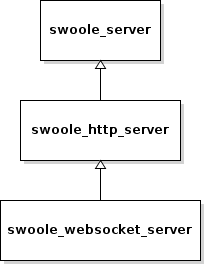
\includegraphics[scale=0.5]{swoole_server.png}
\caption{swoole\_websocket\_server的继承关系}
\end{figure}



下面的示例使用Swoole来实现一个异步非阻塞多进程的WebSocket服务器。

\begin{lstlisting}[language=PHP]
$server = new swoole_websocket_server("0.0.0.0",9501);

$server->on('open',function(swoole_websocket_server $server,$request){
	echo "server: handshake success with fd{$request->fd}\n";
});

$server->on('message',function(swoole_websocket_server $server,$frame){
	echo "receive from {$frame->fd}:{$frame->data}, opcode:{$frame->opcode},fin:{$frame->finish}\n"
	$server->push($frame->fd,"this is server");
});

$server->on('close',function($ser,$fd){
	echo "client {$d} closed\n";
});

$server->start();
\end{lstlisting}

\begin{compactitem}
\item 设置了onRequest回调,websocket服务器也可以同时作为http服务器
\item 未设置onRequest回调,websocket服务器收到http请求后会返回http 400错误页面
\end{compactitem}

\section{onHandShake}

WebSocket建立连接后进行握手,而且WebSocket服务器已经内置了handshake。

如果用户希望自己进行握手处理,可以设置onHandShake事件回调函数。





\begin{lstlisting}[language=PHP]
function onHandShake(swoole_http_request $request, swoole_http_response $response)
\end{lstlisting}

onHandShake事件回调是可选的,而且在设置onHandShake回调函数后不会再触发onOpen事件,需要应用程序代码自行处理。

\section{onOpen}

当WebSocket客户端与服务器建立连接(connect)并完成握手(handshake)后会回调onOpen函数。


\begin{lstlisting}[language=PHP]
function onOpen(swoole_websocket_server $svr,swoole_http_request $req)
\end{lstlisting}

注意,onOpen函数的第2个参数\texttt{swoole\_http\_request \$req}是从1.7.14开始的,之前是\texttt{\$fd}。

\begin{compactitem}
\item \texttt{\$req}是一个Http请求对象,包含了客户端发来的握手请求信息;
\item onOpen事件函数中可以调用push向客户端发送数据或者调用close关闭连接;
\item onOpen事件回调是可选的。
\end{compactitem}

\section{onMessage}

当服务器收到来自客户端的数据帧时会回调onMessage函数。



\begin{lstlisting}[language=PHP]
function onMessage(swoole_server $server, swoole_websocket_frame $frame)
\end{lstlisting}

\begin{compactitem}
\item \texttt{\$frame} 是swoole\_websocket\_frame对象,包含了客户端发来的数据帧信息;
\item onMessage回调必须被设置,不设置onMessage回调则服务器将无法启动。
\end{compactitem}

\subsection{swoole\_websocket\_frame}

swoole\_websocket\_frame共有4个属性,分别是:

\begin{compactitem}
\item \texttt{\$frame->fd},客户端的socket id,使用\texttt{\$server->push}推送数据时需要用到。
\item \texttt{\$frame->data},数据内容,可以是文本内容也可以是二进制数据,可以通过opcode的值来判断。
\item \texttt{\$frame->opcode},WebSocket的OpCode类型,可以参考WebSocket协议标准文档。
\item \texttt{\$frame->finish}, 表示数据帧是否完整,一个WebSocket请求可能会分成多个数据帧进行发送。
\end{compactitem}

如果\texttt{\$data}是文本类型,那么编码格式必然是UTF-8,这是WebSocket协议规定的。

\subsection{OpCode}


\begin{compactitem}
\item \texttt{WEBSOCKET\_OPCODE\_TEXT = 0x1},文本数据
\item \texttt{WEBSOCKET\_OPCODE\_BINARY = 0x2},二进制数据
\end{compactitem}

\section{push}

\texttt{swoole\_websocket\_server->push}用于向websocket客户端连接推送数据,长度最大不得超过2M。


\begin{lstlisting}[language=PHP]
function swoole_websocket_server->push(int $fd, string $data, int $opcode=1,bool $finish=true)
\end{lstlisting}

\begin|{compactitem}
\item \texttt{\$fd}是客户端连接的ID,如果指定的\texttt{\$fd}对应的是TCP连接而不是websocket客户端,那么将会发送失败。
\item \texttt{\$data}是要发送的数据内容。

\item \texttt{\$opcode}用于指定发送数据内容的格式,默认为文本。

如果需要发送二进制内容,则需要设置\$opcode参数为WEBSOCKET\_OPCODE\_BINARY\_FRAME。

\item 如果发送成功返回true,发送失败则返回false。

\end{compactitem}


在实际应用中,如果Websocket服务器需要向所有连接的客户端发送广播通知消息,则可以使用foreach循环来实现。


\begin{lstlisting}[language=PHP]
foreach($server->connections as $fd){
	$server->push($fd,json_encode($data));
}
\end{lstlisting}


\subsection{Frame Type}


WebSocket数据帧类型

\begin{compactitem}
\item \texttt{WEBSOCKET\_OPCODE\_TEXT = 0x1},UTF-8文本字符数据
\item \texttt{WEBSOCKET\_OPCODE\_BINARY = 0x2},二进制数据
\end{compactitem}


\subsection{Connection State}

WebSocket连接状态

\begin{compactitem}
\item \texttt{WEBSOCKET\_STATUS\_CONNECTION = 1},连接进入等待握手
\item \texttt{WEBSOCKET\_STATUS\_HANDSHAKE = 2},正在握手
\item \texttt{WEBSOCKET\_STATUS\_FRAME = 3},已握手成功等待浏览器发送数据帧
\end{compactitem}



\begin{lstlisting}[language=PHP]

\end{lstlisting}



\begin{lstlisting}[language=PHP]

\end{lstlisting}



\begin{lstlisting}[language=PHP]

\end{lstlisting}




\begin{lstlisting}[language=PHP]

\end{lstlisting}




\begin{lstlisting}[language=PHP]

\end{lstlisting}




\begin{lstlisting}[language=PHP]

\end{lstlisting}




\begin{lstlisting}[language=PHP]

\end{lstlisting}



\begin{lstlisting}[language=PHP]

\end{lstlisting}



\begin{lstlisting}[language=PHP]

\end{lstlisting}




\begin{lstlisting}[language=PHP]

\end{lstlisting}




\begin{lstlisting}[language=PHP]

\end{lstlisting}




\begin{lstlisting}[language=PHP]

\end{lstlisting}





\begin{lstlisting}[language=PHP]

\end{lstlisting}



\begin{lstlisting}[language=PHP]

\end{lstlisting}



\begin{lstlisting}[language=PHP]

\end{lstlisting}




\begin{lstlisting}[language=PHP]

\end{lstlisting}




\begin{lstlisting}[language=PHP]

\end{lstlisting}




\begin{lstlisting}[language=PHP]

\end{lstlisting}




\begin{lstlisting}[language=PHP]

\end{lstlisting}



\begin{lstlisting}[language=PHP]

\end{lstlisting}



\begin{lstlisting}[language=PHP]

\end{lstlisting}




\begin{lstlisting}[language=PHP]

\end{lstlisting}




\begin{lstlisting}[language=PHP]

\end{lstlisting}




\begin{lstlisting}[language=PHP]

\end{lstlisting}





\begin{lstlisting}[language=PHP]

\end{lstlisting}



\begin{lstlisting}[language=PHP]

\end{lstlisting}



\begin{lstlisting}[language=PHP]

\end{lstlisting}




\begin{lstlisting}[language=PHP]

\end{lstlisting}




\begin{lstlisting}[language=PHP]

\end{lstlisting}




\begin{lstlisting}[language=PHP]

\end{lstlisting}





\begin{lstlisting}[language=PHP]

\end{lstlisting}



\begin{lstlisting}[language=PHP]

\end{lstlisting}



\begin{lstlisting}[language=PHP]

\end{lstlisting}




\begin{lstlisting}[language=PHP]

\end{lstlisting}




\begin{lstlisting}[language=PHP]

\end{lstlisting}




\begin{lstlisting}[language=PHP]

\end{lstlisting}




\begin{lstlisting}[language=PHP]

\end{lstlisting}



\begin{lstlisting}[language=PHP]

\end{lstlisting}



\begin{lstlisting}[language=PHP]

\end{lstlisting}




\begin{lstlisting}[language=PHP]

\end{lstlisting}




\begin{lstlisting}[language=PHP]

\end{lstlisting}




\begin{lstlisting}[language=PHP]

\end{lstlisting}




\begin{lstlisting}[language=PHP]

\end{lstlisting}



\begin{lstlisting}[language=PHP]

\end{lstlisting}



\begin{lstlisting}[language=PHP]

\end{lstlisting}




\begin{lstlisting}[language=PHP]

\end{lstlisting}




\begin{lstlisting}[language=PHP]

\end{lstlisting}




\begin{lstlisting}[language=PHP]

\end{lstlisting}





\begin{lstlisting}[language=PHP]

\end{lstlisting}



\begin{lstlisting}[language=PHP]

\end{lstlisting}



\begin{lstlisting}[language=PHP]

\end{lstlisting}




\begin{lstlisting}[language=PHP]

\end{lstlisting}




\begin{lstlisting}[language=PHP]

\end{lstlisting}




\begin{lstlisting}[language=PHP]

\end{lstlisting}






\begin{lstlisting}[language=PHP]

\end{lstlisting}



\begin{lstlisting}[language=PHP]

\end{lstlisting}



\begin{lstlisting}[language=PHP]

\end{lstlisting}




\begin{lstlisting}[language=PHP]

\end{lstlisting}




\begin{lstlisting}[language=PHP]

\end{lstlisting}




\begin{lstlisting}[language=PHP]

\end{lstlisting}






\begin{lstlisting}[language=PHP]

\end{lstlisting}



\begin{lstlisting}[language=PHP]

\end{lstlisting}



\begin{lstlisting}[language=PHP]

\end{lstlisting}




\begin{lstlisting}[language=PHP]

\end{lstlisting}




\begin{lstlisting}[language=PHP]

\end{lstlisting}




\begin{lstlisting}[language=PHP]

\end{lstlisting}